\section{Methods}

In this section, we describe the design and workflow of the \ac{SVT}, including implementation details and dependencies.

As a general overview (\cref{fig:svt_architecture}), the user is first prompted to load a patient's \ac{MRI} that will be used as reference image and a corresponding brain parcellation that must be compatible with the software package used to query the database (\cref{sec:svt_loading}).
% If no patient data are available, a \ac{MNI} template is used \cite{fonov_unbiased_2009}.
Then, a list of pre-defined semiology terms and additional settings compatible with the \ac{API} are displayed, and the user fills in the observed semiologies (\cref{fig:svt_loaded,sec:svt_semiologies}).
Finally, the query is submitted using the \ac{API}, which returns the table of datapoints that is used to generate the 3D \ac{EZ} probability map (\cref{fig:svt_query,fig:svt_case_heatmap,sec:svt_querying,sec:svt_visualization}).
% The implementation details and steps presented above are described in \cref{sec:svt_implementation}, \cref{sec:svt_loading}, \cref{sec:svt_semiologies}, \cref{sec:svt_querying} and \cref{sec:svt_visualization}, respectively.

\begin{figure}[!ht]
  \centering
  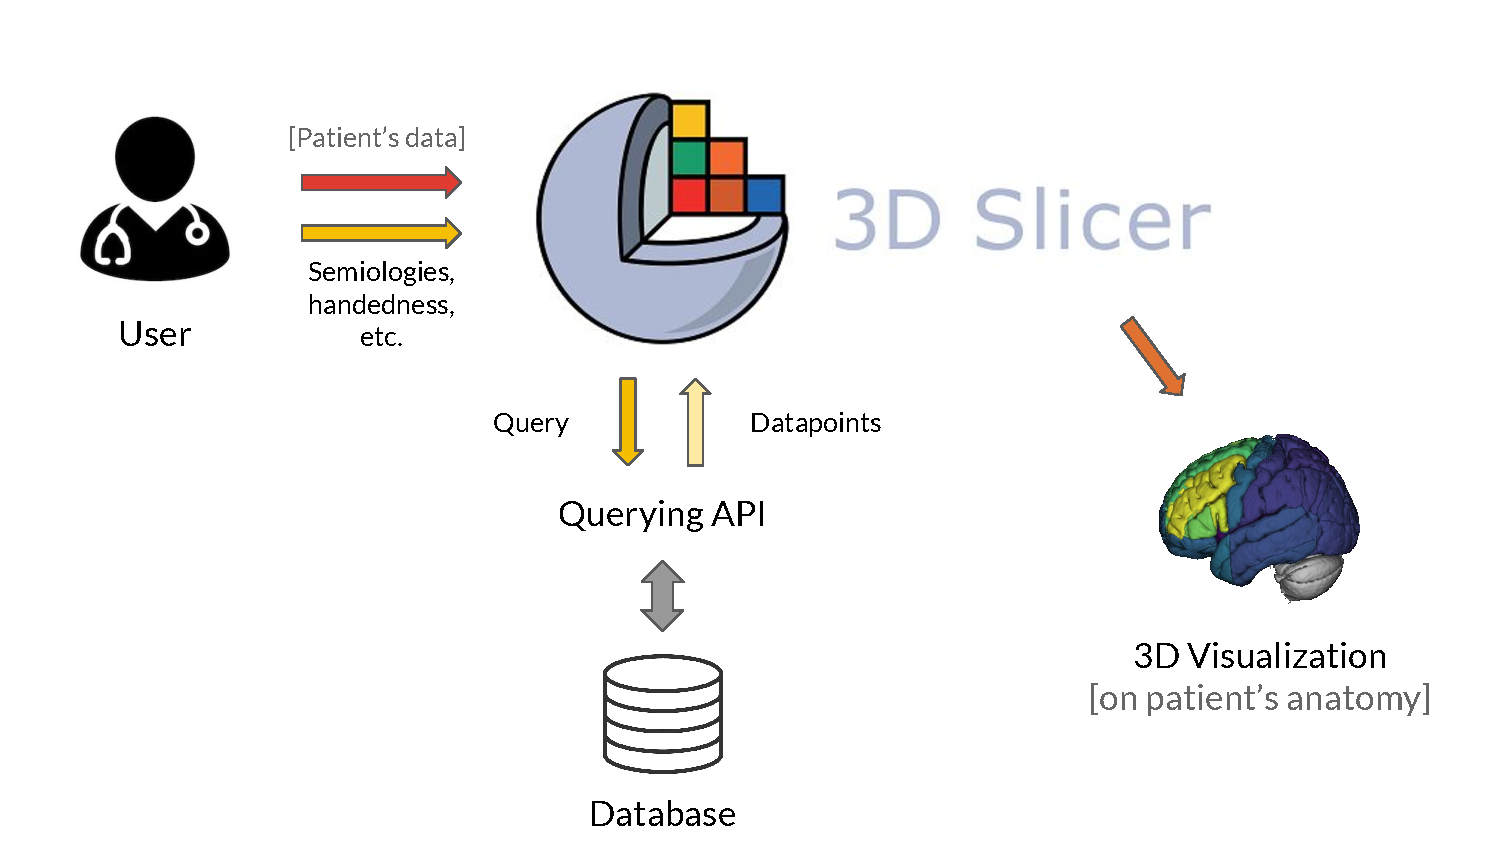
\includegraphics[trim=25 5 25 25, clip, width=0.8\linewidth]{01_svt_diagram}
  \caption[General architecture of the SVT]{
    General architecture of the \ac{SVT}.
    1) The user inputs a list of observed seizure semiologies and (optionally) patient's data comprising an \ac{MRI} and brain parcellation of the patient for visualization in the patient's space.
    2) The \ac{GUI} of the 3D Slicer module is used to input the observed semiologies to the software, without the need to code.
    3) The 3D Slicer module generates a structured query that is sent to be processed by the querying \ac{API} to access the database.
    4) The database is queried and the retrieved datapoints are converted into a \ac{3DMMI} visualization showing the \ac{EZ} probability map overlaid to the patient's anatomy, if provided.
  }
  \label{fig:svt_architecture}
\end{figure}


\subsection{Implementation}
\label{sec:svt_implementation}

The \ac{SVT} is a 3D Slicer Python module \cite{fedorov_3d_2012}.
3D Slicer is ``a free, open source and multi-platform software package widely used for medical, biomedical, and related imaging research''%
\fnurl{https://www.slicer.org/}.
As with 3D Slicer, the \ac{SVT} can be used on all major platforms: Windows, Linux and macOS.

The \ac{SVT} leverages the libraries on which 3D Slicer is built:
\ac{ITK} for image processing \cite{mccormick_itk_2014},
\ac{VTK} for visualization \cite{schroeder_visualization_2006}
and Qt for the cross-platform \ac{GUI}%
\fnurl{https://www.qt.io}.

The Python code for the \ac{SVT} is available on GitHub%
\fnurl{\svtgithubtagged}.
We have also developed a light-weight online version hosted on Binder \cite{bussonnier_binder_2018}, which does not require installation of 3D Slicer and can be accessed through a web browser%
\fnurl{\svtweb}.


\subsection{Dependencies}
\label{sec:svt_dependencies}

The \ac{SVT} depends on an external \ac{API} that must be able to provide the following:
\begin{enumerate}
  \item At start-up, a list of pre-defined semiologies that are used to generate the \ac{GUI} and a list of additional settings to perform the database query.
  \item After the database is queried with a list of semiologies and additional settings, a table with datapoints associated with each brain structure.
\end{enumerate}

The usage examples in this paper use the \svtdatabase database and the corresponding developed software to query the database \cite{alim-marvasti_cortical_2022} (under review) \cite{alim-marvasti_probabilistic_2022}, which were defined according to the Neuromorphometrics atlas parcellation scheme%
\fnurl{http://www.neuromorphometrics.com}.

To query the \svtdatabase database, in this work we used the \texttt{mega\_analysis} package, which can be installed using \ac{PIP} \cite{alim-marvasti_cortical_2022}.
The \texttt{mega\_analysis} software package is installed within the 3D Slicer Python environment in the background, when loading the module, unless it was already installed.


\subsection{Data loading}
\label{sec:svt_loading}

The user is asked to load the patient's \ac{MRI} and a corresponding brain parcellation.
The default behavior when the user opts not to load imaging data, or the \ac{SVT} is being used to explore the database and not for surgical planning, is to load a generic \ac{MNI} template \cite{fonov_unbiased_2009}.
As the \ac{EZ} is expected to be in the gray matter, the brain parcellation is automatically stripped of white matter and other irrelevant structures such as \ac{CSF}, brainstem and cerebellum, for visualization and reporting purposes.
The input brain parcellation must be chosen based on the parcellation scheme in the database being queried.
In this work, we use the \svtdatabase database, which uses the Neuromorphometics atlas integrated in the \ac{GIF} parcellation tool \cite{cardoso_geodesic_2015}.
However, the \ac{SVT} is agnostic to the atlas choice.

Finally, a Slicer segmentation node is instantiated from the parcellation label map and 3D meshes are generated for visualization using the marching cubes algorithm \cite{lorensen_marching_1987,pinter_polymorph_2019}.
The user is then presented with the preprocessed data (\cref{fig:svt_loaded}).

\begin{figure}
  \centering
  \svtscreenshot{02_svt_loaded}
  \caption[SVT after loading a template and its parcellation]{
    Semiology visualization module after loading an \ac{MNI} template as image reference and its corresponding brain parcellation.
    Left: main panel containing a list of suggested semiology terms to be selected by the user;
    right: images in the patient's space.
    Images are shown using the radiological convention, i.e., the left hemisphere is shown on the right and vice versa.
  }
  \label{fig:svt_loaded}
\end{figure}


\subsection{Input semiologies}
\label{sec:svt_semiologies}

Once the image data have been loaded, the pre-defined list of common semiologies is shown on the left-hand side of the screen (\cref{fig:svt_loaded,fig:svt_semiologies}).
Certain semiologies such as \textit{Head version} require a laterality (left or right).
Semiologies such as \textit{Hypermotor} are allowed to have no associated laterality, indicating it was observed for both sides.
Some semiologies such as \textit{Ictal speech} never have an associated laterality.
The dominant hemisphere may also be specified if known, helping to narrow results.

\begin{figure}
  \centering
  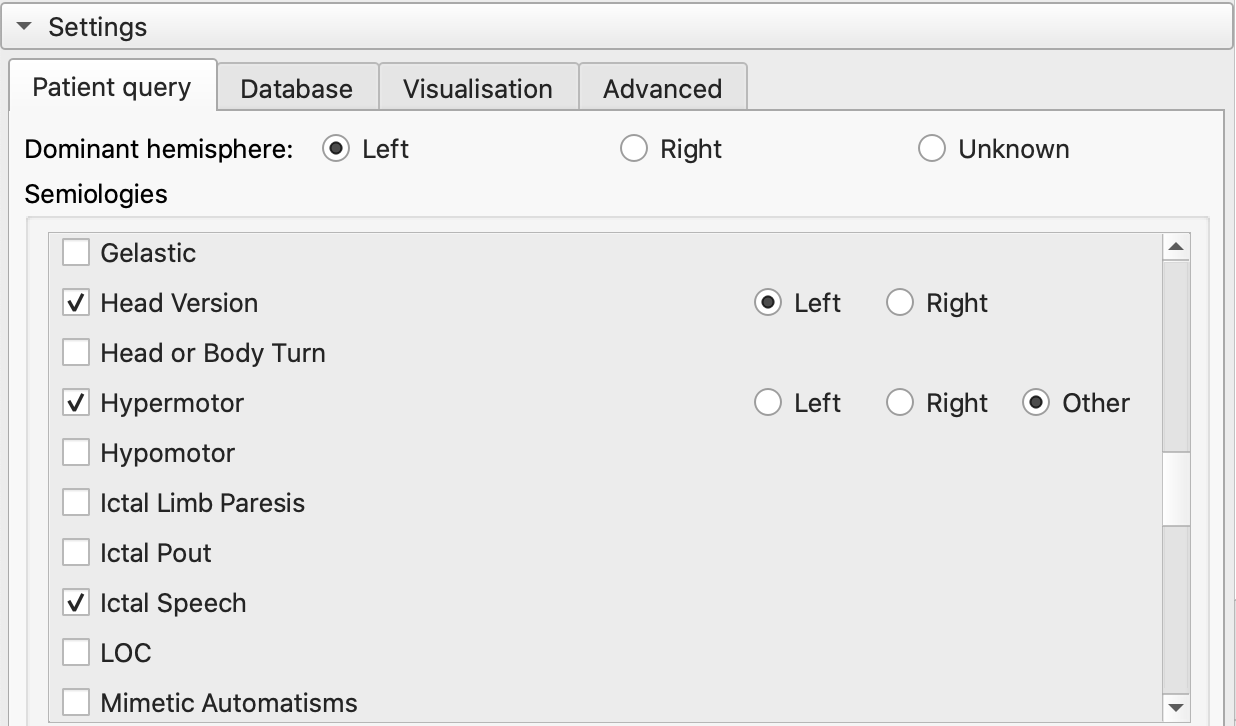
\includegraphics[width=0.8\linewidth]{03_svt_semiologies}
  \caption[List of pre-defined semiologies in the GUI]{
    List of pre-defined semiologies in the \ac{GUI}.
    Users can select a semiology in the list or add a custom one.
    Custom semiologies are matched to a pre-defined semiology using regular expressions to map concepts associated with that semiology.
  }
  \label{fig:svt_semiologies}
\end{figure}

Additionally, the \texttt{mega\_analysis} querying \ac{API} allows for custom semiologies to be entered, which may be matched to one of the pre-defined semiologies using regular expressions \cite{alim-marvasti_cortical_2022} (under review).
Matching is performed in real time within the \ac{GUI} whenever the characters in the widget are modified, as long as three or more characters have been entered (\cref{fig:svt_custom}).
% [If there is no match, no semiologies are suggested]

\begin{figure}
  \centering
  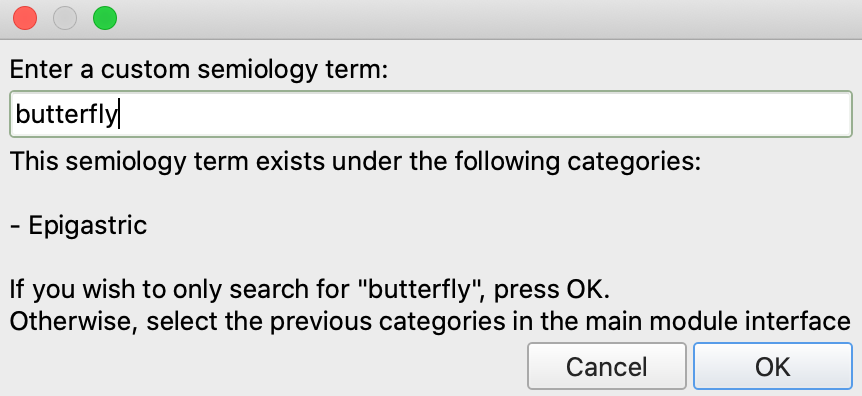
\includegraphics[width=0.65\linewidth]{04_svt_custom_no_shadow}
  \caption[Adding a custom semiology to the semiology visualization module]{
    Adding a custom semiology term to the semiology visualization module.
    For example, `butterflies' and `déjà vu' would be matched with epigastric and psychic auras, respectively.
    In this case, the term \textit{butterfly} was entered as the patient described ``a butterfly feeling in my stomach''.
    The module used to query the database matches the input term with the \textit{Epigastric} semiology term, and therefore the 3D Slicer module suggests matching \textit{Epigastric} to the list of selected semiologies.
  }
  \label{fig:svt_custom}
\end{figure}


\subsection{Querying the database}
\label{sec:svt_querying}

The \ac{SVT} reads the user specified semiologies and settings from the \ac{GUI} and generates a machine-readable data structure to query the database.
As the waiting time to query the database is sometimes in the order of tens of seconds, previous query results are cached in the disk for faster retrieval using \ac{YAML}, a human-readable file format.
The result from querying the database is a table containing the number of datapoints for each brain structure (\cref{tab:single_semiology}).
If multiple semiologies are selected, results are combined and a number between 0 and 1 is computed for each brain structure by the database query package (in this work, \texttt{mega\_analysis}).
Details on how the datapoints for multiple semiologies are combined can be found in \cite{alim-marvasti_cortical_2022} (under review).


\subsection{Visualization}
\label{sec:svt_visualization}

Results from the database query are shown to the user in two ways: a table and a rendering leveraging the brain parcellation image loaded by the user.
The datapoints table is displayed on the \ac{GUI} and the list of structures is sorted by the number of datapoints, showing first the structures with the highest number of datapoints in the database (\cref{fig:svt_query,fig:svt_case_heatmap}).

\begin{figure}
  \centering
  \svtscreenshot{05_svt_query}
  \caption[Results of querying the database with the \textit{Epigastric} semiology]{
    Results of querying the database with the \textit{Epigastric} semiology.
    Left: table showing the number of datapoints associated with each brain structure;
    right: \ac{EZ} probability map, where brightness (and opacity, on the 2D views) is linearly proportional to the number of datapoints.
  }
  \label{fig:svt_query}
\end{figure}

A probability map showing the datapoints per brain parcellation label is generated and displayed on the 2D slice views and the 3D view.
The 2D slice views are centered on the brain structure with the highest number of associated datapoints.
Brain structures without datapoints are hidden from the 2D slice views and shown in gray on the 3D view.
To emphasize the importance of brain structures with a high number of datapoints, the opacity of each structure on the 2D slice views is adjusted to be linearly proportional to the number of associated datapoints.
We chose the open-source, perceptually uniform, sequential colormap \textit{viridis} as default for this application.
This implies that the brightness of each structure is also linearly proportional to the number of associated datapoints.
Other colormaps are available as a user-selectable option, if desired.
The colorbars on the 2D slice views help create a mental mapping from colors to number of datapoints (\cref{fig:svt_query,fig:svt_advanced,fig:svt_case_heatmap}).

\begin{figure}
  \centering
  \svtscreenshot{06_svt_advanced}
  \caption[Demonstration of advanced visualization settings]{
    Demonstration of advanced visualization settings.
    The selected settings are:
    show only the right hemisphere,
    center the views on the right thalamus,
    set minimum opacity to 75\% (default is 25\%)
    and enable color-blind mode.
  }
  \label{fig:svt_advanced}
\end{figure}

\begin{figure}
  \centering
  \svtscreenshot{07_svt_case_heatmap}
  \caption[Querying the database using data from a retrospective patient case]{
    Querying the database using data from a retrospective patient case.
    The selected semiology term was \textit{Head version (right)}, and the dominant hemisphere was \textit{Left}.
    The regions with highest numbers of datapoints concentrate around the left frontal lobe (represented on the right side of the axial and coronal views).
  }
  \label{fig:svt_case_heatmap}
\end{figure}

Advanced visualization settings may be selected by the users.
Settings include
showing only one hemisphere on the 3D view,
setting the minimum opacity on the 2D views or
enabling color blind mode, in which the color-blind-friendly \textit{cividis} colormap is used \cite{nunez_optimizing_2018} (\cref{fig:svt_advanced}).
